\hfill

\chapter{Testing}

\section{Test}

\subsection{Test}

\paragraph{Einsteinsche Formeln:} $\boxed{E = mc^2}$ mit $E$ Energie, $m$ Masse, $c$ Lichtgeschwindigkeit


\begin{wrapfigure}{r}{0.4\columnwidth}
	\pgfplotsset{
		tick label style={font=\tiny},
		label style={font=\tiny},
		legend style={font=\tiny},
		width=0.45\columnwidth,
		compat=1.9
	}
	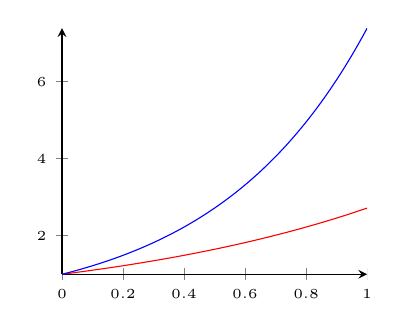
\begin{tikzpicture}
	\begin{axis}[
	axis lines = left,
	%xlabel = $x$,
	%ylabel = {$f(x)$},
	]
	%Below the red parabola is defined
	\addplot [
	domain=0:1, 
	samples=100, 
	color=red,
	]
	{e^x};
	%\addlegendentry{$e^x$}
	%Here the blue parabloa is defined
	\addplot [
	domain=0:1, 
	samples=100, 
	color=blue,
	]
	{e^(2*x)};
	%\addlegendentry{$e^{2x}$}
	
	\end{axis}
	\end{tikzpicture}
\end{wrapfigure}

\paragraph{Einsteinsche Formeln:} mit $E$ Energie, $m$ Masse, $c$ Lichtgeschwindigkeit
\\
Das ist ein Text. Das ist ein Text. Das ist ein Text. Siehe (\ref{testlabel}).
$$\boxed{E = mc^2 = \int_{t_1}^{t_2} \ln (\tau) \, \textnormal{d} \tau}$$
Das ist ein Text. Das ist ein Text. Das ist ein Text.
$$\boxed{E = mc^2 = \int_{t_1}^{t_2} \ln (\tau) \, \textnormal{d} \tau}$$
Das ist ein Text. Das ist ein Text. Das ist ein Text.
Das ist ein Text. Das ist ein Text. Das ist ein Text.

\subsubsection{Einige Einheiten}
\SI{10}{\kilogram} \\
\SI{10.012}{\micro\joule\per\kelvin\tothe{3}}

$\boxed{E = mc^2}$

Das ist ein Text.
%
\begin{equation} \label{testlabel}
\boxed{c_i = \langle\psi|\phi\rangle} \quad  \textnormal{\footnotesize $\psi=$  \SI{10.023e-31}{\pascal}}
\end{equation}
%\begin{empheq}[box=\mathbox]{equation} 
%c_i = \langle\psi|\phi\rangle, \quad  \textnormal{\footnotesize $\psi=$  \SI{10.023e-31}{\pascal}}
%\end{empheq}
Wobei: $\psi=$ \SI{10.023e-31}{\pascal}
%
$$ \vec{v}_A = \vec{v}_A + \vec{\omega} \times \vec{r}_{AB} \Rightarrow \doubleunderline{v_{A_x} = 2v}, \textnormal{wobei } v = \SI{1.5}{\meter \per \second}$$


\begin{equation*}
	\text{Pr} = \frac{\nu_L}{a_L}
\end{equation*}


\begin{empheq}[box =\widecolourbox]{equation*}
{\text{Re} = \frac{\rho u D}{\mu}} = \frac{\text{num}}{\text{den}} \qquad \text{\emph{kinematic viscosity}: } {\nu = \frac{\mu}{\rho}}
\end{empheq}


\section{Classes of Optimization Problems}

\subsection{Dynamic vs.\ Static}
\paragraph{Static optimization} \emph{Finite} number of optimization variables.
\paragraph{Dynamic optimization} \emph{Infinite} number of optimization variables. Determines a function of an independent variable (often time) $\to$ optimization over function space. Example: Optimal control problem.

\subsection{Linear Programming (LP)}
\begin{equation*}
\boxed{\min_{\vec x} \vec c^T \vec x \qquad \text{subject to }  \vec{Ax} - \vec{b} = \vec 0, \, \vec x \geq \vec 0}
\end{equation*}
\begin{itemize}
	\item linear objective function
	\item linear/affine constraints
	\item \emph{always convex}
\end{itemize}

\subsection{Quadratic Programming (QP)}
\begin{equation*}
\boxed{\min_{\vec x} \frac{1}{2} \vec x^T \vec H \vec x + \vec x^T \vec q\qquad \text{subject to } \vec{Ax} - \vec{b} = \vec 0, \, \vec{Cx} - \vec d \leq \vec 0}
\end{equation*}
\begin{itemize}
	\item quadratic objective function
	\item linear/affine constraints
	\item \emph{convex if $\vec H$ is positive semi-definite}
\end{itemize}

\subsection{Nonlinear Programming (NLP)}
\begin{equation*}
\boxed{\min_{\vec x} J(\vec x) \qquad \text{subject to } \vec{h}(\vec x) = \vec 0, \, \vec g(\vec x) \geq \vec 0}
\end{equation*}
\begin{itemize}
	\item cost function or constraints are nonlinear
	\item \emph{in general non-convex}
\end{itemize}

\subsection{Integer Programming (IP)}
\begin{equation*}
\boxed{\min_{\vec x} \vec c^T \vec x \qquad \text{subject to } \vec{Ax} - \vec{b} = \vec 0, \, \vec x \in \mathbb Z_{+}^n}
\end{equation*}
\begin{itemize}
	\item variables are integer
	\item \emph{integer optimization problem}
\end{itemize}

\section{Convexity}



\subsection{Convex Sets}

Set $\mathcal{X} \subseteq \mathbb R^n$ is convex, if for random point $\vec x, \vec y \in \mathcal{X}$:
\begin{equation*}
\vec z = k \vec x + (1 - k)\vec y \in \mathcal{X} \forall k \in [0, 1]
\end{equation*}

\paragraph{Geometric Interpretation} A set is convex if the connecting line between two random points inside the feasible set lies completely inside the set.


\subsection{Convex Functions}

A function $f:\mathcal{X} \to \mathbb R$ is convex, iff $\mathcal{X}$ is convex and for random points $\vec x, \vec y \in \mathcal{X}, \vec \neq \vec y$ and $\vec z = k \vec x +(1-k)\vec y$:
\begin{equation*}
f(\vec z) \leq kf(\vec x) + (1 - k)f(\vec y) \forall k \in [0, 1]
\end{equation*}

\paragraph{Geometric Interpretation} A function is convex, if the connecting line between two random points on the function is always above or at most on the function value itself.

For twice differentiable functions, it holds: 
\begin{itemize}
	\item $f(\vec x)$ is convex, iff $\vec H(\vec x)$ is positive \emph{semi}-definite $\forall \vec x in \mathcal{X}$ and $\mathcal{X}$ is convex
	\item $f(\vec x)$ is \emph{strictly} convex, iff $\vec H(\vec x)$ is positive definite $\forall \vec x in \mathcal{X}$ and $\mathcal{X}$ is convex.
\end{itemize}

\subsection{Convex Optimization Problem}

Cost function convex + feasible set convex $\Rightarrow$ optimization problem convex

Convex problems: Every local minimum is also a global minimum!

\section{Optimality Conditions for Nonlinear Programs}

\subsection{Unconstrained}
\begin{equation*}
\boxed{\min_{\vec x \in \mathbb R^n} J(\vec x)}
\end{equation*}

\paragraph{1st Order \emph{Necessary} Condition (Local) Minimum} $\grad J(\vec x^\ast) = \vec 0$

\paragraph{2nd Order \emph{Sufficient} Condition (Local) Minimum} $\grad^2 J(\vec x^\ast)  \succ 0$\\ (positive (semi-)definite Hessian)


\subsection{With Equality Constraints}
\begin{equation*}
\boxed{\min_{\vec x \in \mathbb R^n} J(\vec x) \qquad \vec{h}(\vec x) = \vec 0 \qquad \vec h:\mathbb R^n \to \mathbb R^p}
\end{equation*}

\paragraph{Lagrange Function}
\begin{equation*}
L(\vec x, \vec \lambda) = J(\vec x) + \vec \lambda^T \vec h(\vec x)
\end{equation*}
where $\lambda \in \mathbb R^p$: \emph{Lagrange multipliers} or \emph{dual variables}

\paragraph{1st Order \emph{Necessary} Condition (Local) Minimum (simplified KKT)} 
\begin{equation*}
\grad L(\vec x^\ast, \vec \lambda^\ast) = 
\begin{bmatrix}
\grad_{\vec x} L(\vec x^\ast, \vec \lambda^\ast) \\
\grad_{\vec \lambda} L(\vec x^\ast, \vec \lambda^\ast)
\end{bmatrix} =
\begin{bmatrix}
\grad J(\vec x^\ast) + \grad \vec h(\vec x^\ast)\vec \lambda^\ast \\
\vec h(\vec x^\ast)
\end{bmatrix}
= \vec 0
\end{equation*}
If $\grad \vec h(\vec x^\ast)$ has full rank $p$ ($\Leftrightarrow$ linear independent), then every minimizer $\vec x^\ast, \vec \lambda^\ast$ solves $\grad L(\vec x, \vec \lambda) = \vec 0$ (LICQ, linear independence constraint qualification)

\subsection{QP with Affine Equality Constraints}
\begin{equation*}
\boxed{\min_{\vec x} \frac{1}{2} \vec x^T \vec H \vec x + \vec x^T \vec q\qquad \text{subject to } \vec{Ax} - \vec{b} = \vec 0, \, \vec{Cx} - \vec d \leq \vec 0}
\end{equation*}

\paragraph{Lagrange Function} $L(\vec x, \vec \lambda) = J(\vec x) + \vec \lambda^T(\vec A \vec x - \vec b)$

\paragraph{1st Order \emph{Necessary} Condition for (Local) Minimum}
\begin{equation*}
\grad L = \vec 0 \Leftrightarrow 
\underbrace{\begin{bmatrix}
	\vec H &\vec A^T \\
	\vec A & \vec 0
	\end{bmatrix}}_{\text{\emph{KKT-Matrix}}}
= 
\begin{bmatrix}
-\vec q \\
\vec b
\end{bmatrix}
\end{equation*}

\subsection{Equality and Inequality Constraints}
\begin{equation*}
\boxed{\min_{\vec x \in \mathbb R^n} J(\vec x) \qquad \text{subject to: } h_i (\vec x) = 0, i \in \vec{\mathcal{E}}, \quad g_i(\vec x) \leq 0, i\in \vec{\mathcal J}}
\end{equation*}
\paragraph{Lagrange Function}
\begin{equation*}
L(\vec x, \vec \lambda) = J(\vec x) + \sum_{i \in \vec{\mathcal{E}}} \lambda_i h_i + \sum_{i \in \vec{\mathcal{J}}} \mu_i g_i = J(\vec x) + \vec \lambda^T \vec h(\vec x) + \vec mu^T \vec g(\vec x)
\end{equation*}
\paragraph{Active Set} $\vec{\mathcal A} = \vec{\mathcal E} \cup \{ i \in \vec{\mathcal{J}} | g_i(\vec x)  = 0 \}$

\paragraph{1st Order \emph{Necessary} Conditions (KKT conditions) for Local Minimum} \emph{Sufficient} for convex problems, otherwise only \emph{necessary}.
\begin{itemize}
	\item Primal feasibility: $h_i(\vec x^\ast) = 0, i \in E \qquad g_i(\vec x^\ast) \leq 0, i \in I$
	\item Dual feasibility: $\grad_{\vec x} L (\vec x^\ast, \vec \lambda^\ast, \vec \mu^\ast) = 0 \qquad \mu_i^\ast \geq 0, i \in I$
	\item Complementary slackness: $\mu_i^\ast g_i(\vec x^\ast) = 0, i \in I$
\end{itemize}
where:
$
\grad_{\vec x}L(\vec x^\ast, \vec \lambda^\ast, \vec \mu^\ast) = \grad f(\vec x^\ast) + \sum_{i \in {{E}}} \lambda_i \grad h_i(\vec x^\ast) + \sum_{i \in {{I}}} \mu_i \grad g_i(\vec x^\ast) = 0
$
